% !TEX root =  master.tex
\chapter{Fazit und Ausblick}
\section{Zusammenfassung der Analyseergebnisse}
\label{fazit}
Die Ergebnisse der innerhalb der vorliegenden Thesis durchgeführten Evaluationen der aktuell auf der \ac{CF} basierenden Infrastrukturlösung und des Kubernetes Prototyps sind in der Abbildung \ref{fazit_tabelle} gegenübergestellt.
Dabei bedeutet die Bewertung mit einem \textbf{+}, dass die entsprechende Plattform im jeweiligen Merkmal Vorteile gegenüber der mit einem \textbf{-} oder mit einer \textbf{0} markierten Plattform hat. Die Bewertung \textbf{0} entspricht hierbei einer neutralen Bewertung. Dies bedeutet, dass bei der Verwendung der Plattform in diesem Punkt keine generellen Probleme bestehen, sondern lediglich die verglichene Plattform bessere Funktionalitäten bereitstellt. Des Weiteren wurden die in Kapitel \ref{gewichtung_merkmale} seitens des Infrastruktur-Teams stärker gewichteten Merkmale in der Farbe blau dargestellt.
\\
\begin{figure}[h]
	\begin{center}
		\includegraphics[width=16cm]{img/fazit_tabelle.PNG}
		\caption[Zusammenfassung der Evaluationen von \acl{CF} und Kubernetes]{Zusammenfassung der Evaluationen von \acl{CF} und Kubernetes}
		\label{fazit_tabelle}
	\end{center}
\end{figure}
\\
Innerhalb der Untersuchung der Performance der beiden Plattformen konnten keine bemerkenswerten Unterschiede festgestellt werden.\\
\newpage
Jedoch können, wie der Abbildung \ref{grafik_kostenvergleich} zu entnehmen ist, durch die Portierung der Anwendungsumgebung der Softwarelösung auf ein Kubernetes Cluster innerhalb des SAP Subscription Billing Projektes monatliche Betriebskosten in Höhe von 4.670,98\textrm{\euro} eingespart werden. Dies entspricht einer Verringerung der Kosten um 44,13\%.\\
\\
\begin{figure}[h]
	\begin{center}
		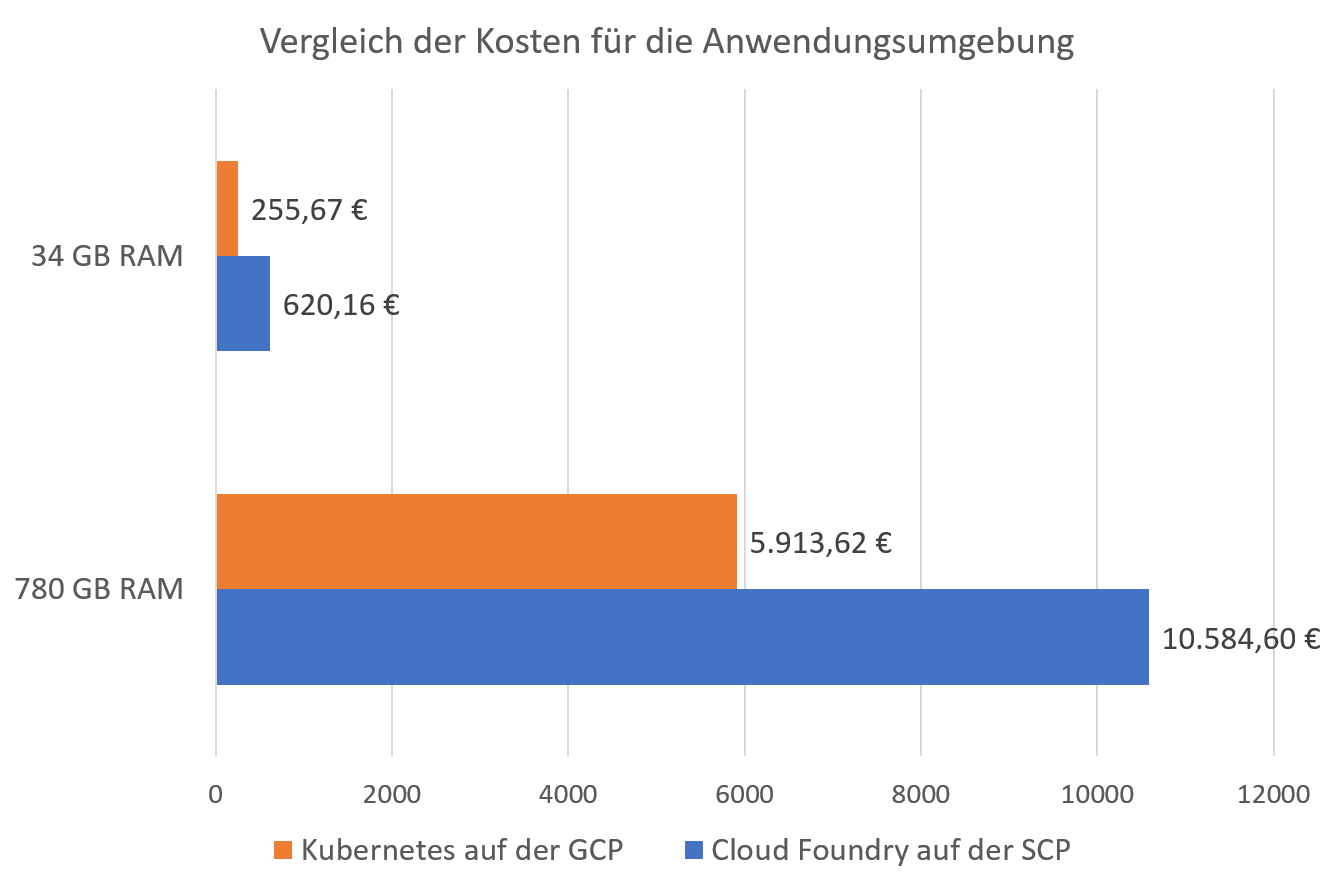
\includegraphics[width=14cm]{img/Kostenvergleich.png}
		\caption[Kostenvergleich Anwendungsumgebung für \acs{CF} und Kubernetes]{Kostenvergleich Anwendungsumgebung für \acl{CF} und Kubernetes}
		\label{grafik_kostenvergleich}
	\end{center}
\end{figure}
\\
Des Weiteren erfolgt die generelle Kostenberechnung der \ac{GCP} ausschließlich auf den tatsächlich konsumierten Infrastrukturressourcen. Im Vergleich dazu werden innerhalb des SAP Subscription Billing Projektes die Gebühren der von der \ac{SCP} angebotenen \ac{CF}-Umgebung unabhängig von dem tatsächlichen Verbrauch berechnet. Hierbei fallen seitens der \ac{SCP} feste monatliche Kosten an.\\
Auch der Vergleich der Sicherheitskonzepte der beiden Plattformen hat gezeigt, dass durch das standardmäßige Nichtvorhandensein von extern verfügbaren Endpunkten keine zusätzlichen Sicherheitsvorkehrungen zur Absicherung der Schnittstellen benötigt werden. Zudem stellte sich die automatische Verwendung von \ac{mTLS} innerhalb des Kubernetes Clusters für die Absicherung der Kommunikation als sehr hilfreich heraus.\\
Da die Verfügbarkeit der beiden Plattformen hauptsächlich von der Verfügbarkeit des zugrundeliegenden \ac{IaaS}-Providers abhängig ist und zusätzlich weitere Abhängigkeiten, wie beispielsweise die Verfügbarkeit der verwendeten Datenbanken existieren, konnte kein klarer Unterschied bezüglich der Verfügbarkeit der beiden Plattformen festgestellt werden.\\
Allerdings zeichnet sich Kubernetes besonders durch die Möglichkeiten der dynamischen Skalierung aus. Hierbei unterstützt Kubernetes sowohl die automatische horizontale als auch vertikale Skalierung auf der Pod-Ebene oder auch die gesamte Skalierung der für das Cluster bereitgestellten Rechenressourcen des \ac{IaaS}-Providers.\\
Die \ac{CF} hingegen unterstützt mit Hilfe des App-Autoscaler-Projekt zwar die dynamische vertikale Skalierung einer Anwendung, jedoch kann die horizontale Skalierung ausschließlich manuell und nicht automatisiert durchgeführt werden.\\
Generell unterstützt Kubernetes durch die mögliche Konfiguration aller vorhandenen \ac{API}-Objekte sowie den zusätzlich angebotenen Custom Ressource Definitions eine sehr detaillierte Konfiguration des gesamten Kubernetes Clusters als auch der einzelnen Anwendungsbereitstellung. Durch die Verwendung des Service Meshes Istio können besonders im Bereich des Traffic Managements umfangreiche Konfigurationen von Funktionalitäten, wie beispielsweise dem gewichteten Routing der Anfragen, vorgenommen werden, welche bei der \ac{CF} gar nicht unterstützt werden. Außerdem zeigte die innerhalb des SAP Subscription Billing Projektes praktische Verwendung der \ac{CF}, dass aufgrund fehlender Konfigurationsmöglichkeiten Probleme bei dem produktiven Betrieb der Softwarelösung auftreten können. Ein Beispiel dafür ist die nicht konfigurierbare Timeoutzeit der Health Checks.\\
Im Punkt der Erweiterbarkeit bieten die beiden Plattformen mit dem Blue-Green Deployment der \ac{CF} und der Rolling Update Strategie von Kubernetes grundsätzlich sehr ähnliche Strategien für die Aktualisierung der bereitgestellten Anwendungen mit Zero-Downtime an. Generell unterstützt Kubernetes durch das sehr breite Spektrum an vorkonfigurierten Helm Charts die Erweiterung der Infrastrukturlösung um zusätzliche Open Source Tools mit minimalem Aufwand.\\
Die praktische Umsetzung des Kubernetes Prototyps hat gezeigt, dass das hierfür benötigte Vorwissen und die Einarbeitungszeit definitiv höher als bei der \ac{CF} ist, weshalb dies bei einer Portierung der gesamten Softwarelösung berücksichtigt und eingeplant werden sollte.\\
\\
Besonders mit Hilfe des nativ unterstützten Multi Zonen Konzeptes zeichnet sich Kubernetes im Punkt der Portierbarkeit aus. Dabei können Kubernetes Cluster, deren Infrastruktur auf unterschiedlichen \ac{IaaS}-Providern in mehreren Zonen bereitgestellt wird, konzeptioniert und umgesetzt werden. Dahingegen ist eine \ac{CF}-Space immer an eine Zone eines \ac{IaaS}-Providers gebunden. Somit kann die auf der \ac{CF} bereitgestellte Softwarelösung nicht ohne Umstände auf einen anderen \ac{IaaS}-Provider oder in eine andere Zone portiert werden.\\
Anhand der erfolgreichen Ersetzung einiger innerhalb der aktuellen Infrastrukturlösung zusätzlich benötigter Infrastruktur-Services und Komponenten durch native Funktionalitäten und Objekte von Kubernetes und Istio konnte gezeigt werden, dass Kubernetes in dem Vergleichsmerkmal Infrastruktur-Services definitiv vorteilhaft ist. \\
Insgesamt bietet die Kubernetes Plattform besonders in Kombination mit dem Service Mesh Istio bereits sehr viele Funktionalitäten nativ an, welche für den produktiven Betrieb eine Cloud nativen \ac{SaaS}-Lösung benötigt werden. Auch die teilweise innerhalb der Microservices implementierten Funktionalitäten, wie beispielsweise die gegenseitige Authentifizierung der Microservices, werden im Kubernetes Prototyp nicht mehr benötigt und von der Plattform selbst übernommen.\\
Im Punkt der Dienste für das Monitoring- und Logging-Konzept der bereitgestellten Anwendung bieten die von der \ac{SCP} angebotenen Dienste standardmäßige Möglichkeiten, welche keine weiteren Implementierungen oder einen eigenen Betrieb der Tools benötigen. Jedoch zeigte die mittels des Prototyps erfolgreich umgesetzte Implementierung der im SAP Subscription Billing Projekt eingesetzten Tools, dass diese auch für das Kubernetes Cluster implementiert und ohne Limitationen verwendet werden können. Allerdings muss hierbei der Betrieb des ELK Stacks und die Verwaltung und Archivierung der Logdateien selbst übernommen werden. Diese Aufgaben werden innerhalb der Dienste der \ac{SCP} zwar übernommen, jedoch fallen hierfür auch feste monatliche Servicegebühren an.\\
Außerdem konnten besonders durch den Einsatz des Service Meshes Istio zusätzliche Funktionalitäten umgesetzt werden, welche bisher in der aktuellen Infrastrukturlösung nicht möglich gewesen sind. Dazu gehört beispielsweise das Tool \textbf{Kiali}, welches als grafische Webanwendung für die Verwaltung und Steuerung der gesamten Netzwerkkommunikation genutzt werden kann. Ein Ausschnitt der grafischen Darstellung der Netzwerkkommunikation des Kiali Tools ist im Anhang in Abbildung \ref{anhang_kiali_dashboard} zu finden.\\
Des Weiteren implementiert Istio das Tracing Tool \textbf{Jaeger}. Dieses kann für die Nachvollziehbarkeit aufeinander folgender Anfragen verwendet werden. Für dessen Verwendung müssen ausschließlich weitere \ac{HTTP}-Header und die Funktionalität der Weitergabe der \ac{HTTP}-Header in die Microservices eingebaut werden. Eine Anleitung für die praktische Umsetzung der Weitergabe der \ac{HTTP}-Header ist unter dem angegebenen Link zu finden.\footnote{Anleitung Umsetzung Weitergabe \ac{HTTP}-Header: \url{https://istio.io/docs/tasks/observability/distributed-tracing/overview/\#trace-context-propagation}} Jedoch wurde dies aufgrund des beschränkten zeitlichen Rahmens der vorliegenden Thesis nicht umgesetzt und dient ausschließlich zum Aufzeigen weiterer möglichen Funktionalitäten des Service Meshes Istio.\\
\\
Anhand der zuvor zusammengefassten Ergebnisse der Evaluationen der beiden Plattformen sowie durch die erfolgreiche prototypische Portierung der SAP Subscription Billing Lösung auf das Kubernetes Cluster und der dabei umgesetzten Funktionalitäten und zusätzlichen Möglichkeiten kann die am Anfang der vorliegenden Thesis gestellte wissenschaftliche Fragestellung, ob der Einsatz einer containerbasierten Infrastrukturlösung für die Weiterentwicklung und den Betrieb der \ac{SaaS}-Lösung im Bezug zur bisherigen Infrastrukturlösung verbessert werden kann, mit einem ``Ja`` beantwortet werden.\\ 
Dieses Fazit begründet sich auch durch die in Kapitel \ref{gewichtung_merkmale} erläuterte Gewichtung der Merkmale. Dabei sind für das Infrastruktur-Team des Projektes die Merkmale Sicherheit, Verfügbarkeit, Skalierbarkeit, Konfigurierbarkeit, Erweiterbarkeit und Monitoring und Logging für die Begründung der Entscheidung einer Plattform ausschlaggebend. Besonders die Konfigurierbarkeit und Sicherheit der Bereitstellung der \ac{SaaS}-Lösung kann durch die zuvor zusammengefassten Funktionalitäten von Kubernetes und Istio verbessert werden. Generell kann durch das Ersetzen einiger zusätzlicher Infrastruktur-Services und Komponenten insgesamt die Komplexität der Infrastrukturlösung und somit auch der Wartungsaufwand verringert werden.\\ 
Ausschließlich innerhalb der Möglichkeiten für das Management der Logdateien der bereitgestellten Anwendungen existiert für Kubernetes kein standardmäßiges ``as-a-Service``-Angebot, weshalb der ELK-Stack einmalig selbst implementiert und betrieben werden muss. Da dies innerhalb der ausschlaggebenden Merkmale des Infrastruktur-Teams allerdings der einzige Nachteil bei der Verwendung von Kubernetes ist, kann dieser, verglichen mit den umfangreichen Möglichkeiten und den Vorteilen von Kubernetes, vernachlässigt werden und sollte ausschließlich in der Planung der finalen Portierung der \ac{SaaS}-Lösung dementsprechend berücksichtigt werden.\\
\\
Bezüglich der kritischen Reflexion der Ergebnisse der vorliegenden Thesis sollte beachtet werden, dass innerhalb der prototypischen Portierung der \ac{SaaS}-Lösung eine repräsentative Auswahl an Microservices verwendet wurde. Dadurch kann nicht ausgeschlossen werden, dass bei einer Portierung der gesamten Infrastrukturlösung bisher nicht vorhandene Herausforderungen entstehen.\\
Außerdem ist zu berücksichtigen, dass für den Prototyp lokale Instanzen der benötigten Datenbanken auf dem Cluster selbst bereitgestellt wurden. Allerdings werden in der aktuellen Infrastrukturlösung die von der \ac{SCP} angebotenen Dienste für die Bereitstellung und den Betrieb der Datenbanken verwendet. Deshalb sollte für die produktive Portierung entweder eine Integration der gemanagten Datenbanken der \ac{SCP} oder ein Konzept zur eigenen Bereitstellung und Verwaltung der Datenbanken erstellt werden.\\
Zwar wurden aufgrund des Faktes, dass das Kubernetes Cluster ausschließlich für den Prototyp provisioniert und vom Autor der vorliegenden Thesis verwendet wurde, kein Berechtigungskonzept für den Zugriff auf das Kubernetes Cluster benötigt. Allerdings sollte dies bei einer produktiven Verwendung definitiv mit dem in Kapitel \ref{bewertung_k8s_prototyp} erläuterten Sicherheitskonzept für die Absicherung des externen Zugriffs auf das Kubernetes Cluster umgesetzt werden.\\
Des Weiteren basiert der Kostenvergleich der beiden Plattformen ausschließlich auf den für die Application Runtime Umgebung anfallenden Kosten. Hierbei sollte jedoch für einen umfangreichen und repräsentativen Kostenvergleich die Betrachtung der gesamten \ac{TCO} durchgeführt werden.
 
\newpage
\section{Ausblick Infrastrukturlösung SAP Subscription Billing}
\label{ausblick}
Die vorliegende Thesis hat gezeigt, dass die Portierung der SAP Subscription Billing Lösung auf ein Kubernetes Cluster definitiv als sinnvoll betrachtet werden kann. Dies wurde auch bei der Präsentation der Ergebnisse innerhalb des Infrastruktur-Teams des Projektes anerkannt und bestätigt.\\
Jedoch ist besonders die komplette Portierung der \ac{SaaS}-Lösung, insbesondere, da diese bereits bei einigen Kunden produktiv eingesetzt wird, realistisch betrachtet nicht in kurzer Zeit möglich und sollte umfangreich geplant und vorbereitet werden. Allerdings konnte mittels der vorliegenden Thesis erfolgreich bewiesen werden, dass dieser Aufwand durchaus sinnvoll ist.\\
Deshalb sieht der langfristige Plan des SAP Subscription Billing Projektes die schrittweise Portierung der Softwarelösung in ein Kubernetes Cluster vor. Hierbei dient die vorliegende Thesis als essentielle Grundlage, welche die theoretischen Konzepte der Kubernetes Plattform und dem Service Mesh Istio vorstellt sowie exemplarische Implementierungen für deren praktische Verwendung aufzeigt.\\
Ebenso wurde vom Autor der vorliegenden Thesis ein zusätzliches Konzept zur automatischen Portierung aller Microservices der \ac{SaaS}-Lösung erstellt. Dabei wurde eine eigenständige Jenkins-Pipeline implementiert, welche mit Hilfe von Skripts, einem eigens erstellten Helm Chart und dem Skaffold Tool die automatische Bereitstellung aller Microservices und den weiteren benötigten Objekten von Kubernetes und Istio auf das Kubernetes Cluster ermöglicht. Weitere Informationen zu der über den Rahmen der vorliegenden Thesis hinausgehende Umsetzung des zuvor genannten Konzeptes sind im Anhang in Kapitel \ref{anhang_umsetzung_komplettes_Deployment} zu finden.\\

\newpage
\section{Entwicklungsmöglichkeiten von \acs{SaaS}-Lösungen durch Kubernetes}
\label{Entwicklungsmöglichkeiten_Kubernetes_SaaS}
Besonders bei \ac{SaaS}-Lösungen, welche auf einer Microservice-Architektur basieren, existieren einige Herausforderungen, wie beispielsweise benötigte Funktionalitäten für Tracing, Traffic Management oder auch das Berechtigungs- und Sicherheitskonzept für einzelne Mandanten. Diese sind speziell im Cloud nativen Umfeld sehr relevant und prägen sich weiter bei einem weltweiten produktiven Einsatz der \ac{SaaS}-Lösung aus.\\
Um den dabei entstehenden Anforderungen besonders im Bereich der Verfügbarkeit und Skalierbarkeit der Software gerecht werden zu können, bietet Kubernetes grundlegende Mechanismen und Konzepte, wie zum Beispiel die automatische vertikale und horizontale Skalierung auf mehreren Ebenen sowie auch das Multi Zone Konzept für eine regional verteilte Bereitstellung der Softwarelösung, an. Auch die Vision des Cluster Federation Projektes, welches auf die virtuelle Aggregation heterogen bereitgestellter Kubernetes Cluster abzielt, wird mit großer Wahrscheinlichkeit in naher Zukunft sehr relevant werden und eröffnet beispielsweise für einen hybriden Cloudansatz neue Möglichkeiten.\\ 
Dabei können exemplarisch Teile der Softwarelösung, welche aus bestimmten Sicherheitsaspekten besonders geschützt werden müssen, auf einem privaten Cluster, das in eigenen Rechenzentren des Kunden betrieben wird, bereitgestellt werden. Wohingegen die Teile der Softwarelösung, welche eine dynamische und globale Skalierbarkeit benötigen, in einem Public-Cloud Cluster des \ac{SaaS}-Anbieters bereitgestellt werden können. Dieses könnte mittels des Multi Zone Konzeptes auf der Infrastruktur unterschiedlicher \ac{IaaS}-Provider aus regional verteilten Zonen basieren, um die Abhängigkeit eines einzelnen Rechenzentrums des \ac{IaaS}-Providers zu umgehen.\\
Somit unterstützt Kubernetes optimal die Entwicklung und den Betrieb von Cloud nativen \ac{SaaS}-Lösungen. Dadurch rechtfertigt Kubernetes seinen aktuellen Status als Industriestandard für die Orchestration von Containeranwendung und hat mit den geplanten Weiterentwicklungen durchaus Potenzial, diesen Status auch in der Zukunft weiter ausbauen zu können. 
